\chapter{Теоретические сведения}


Дан разрядный контур:
\begin{figure}[H]
    \centering
    \includegraphics[scale=0.7]{data/image/scheme.png}
    \caption{Схема контура.}
\end{figure}
%\includegraphics[scale=1]{scheme.png}

Получена система дифференциальных уравнений:

\begin{equation*}
    \begin{cases}
        L_\text{к}\frac{dI}{dt} + (R_\text{к} + R_p) I - U_c = 0 \\
        C_\text{к} \frac{dU_c}{dt} = -I \\
    \end{cases}
\end{equation*}

Необходимо решить систему и построить графики $I(t), U_c(t), I\cdot R_p(t), R_p(t), T_0(t)$.

Cопротивление газоразрядной трубки, находится в зависимости от силы тока:

\begin{equation*}
    R_p(I) = \frac{l_{\text{э}}}{2 \pi R^2 \int_0^1 \sigma(T(z))zdz}
\end{equation*}

Даны 2 таблицы, для нахождения $T_0, m, \sigma$

Система уравнений решается методом Рунге-Кутта 4 порядка для системы ОДУ.

\begin{equation*}
    y_{n+1} = y_n + \frac{k_1 + 2k_2 + 2k_3 + k_4}{6},
\end{equation*}

\begin{equation*}
    z_{n+1} = z_n + \frac{q_1 + 2q_2 + 2q_3 + q_4}{6}
\end{equation*}

, где

\begin{equation*}
    k_1 = h_n f(y_n, z_n), ~~q_1 = h_n \varphi (y_n)
\end{equation*}

\begin{equation*}
    k_2 = h_n f (y_n + \frac{k_1}{2}, z_n + \frac{q_1}{2}),~~ q_2 = h_n \varphi(y_n + \frac{k_1}{2})
\end{equation*}

\begin{equation*}
    k_3 = h_n f (y_n + \frac{k_2}{2}, z_n + \frac{q_2}{2}), ~~q_3 = h_n \varphi(y_n + \frac{k_2}{2})
\end{equation*}

\begin{equation*}
    k_4 = h_n f (y_n + k_3, z_n + q_3, ~~q_4 = h_n \varphi(y_n + k_3)
\end{equation*}
